%************************************************
\chapter{Stabilization by spatial variation of the drive}\label{ch:metronome-spin}

In this chapter, we consider a clean, i.e. disorder-free, Ising spin chain and explore the influence of a spatially inhomogeneous drive. Remarkably, we find the time dynamics to be very sensitive to even small variations of said drive which we demonstrate by limiting the spatial inhomogeneity of the drive to a single site, while all other sites experience the same driving. 

\newpage
\pdfbookmark[2]{Publication}{metronomespin-paper}
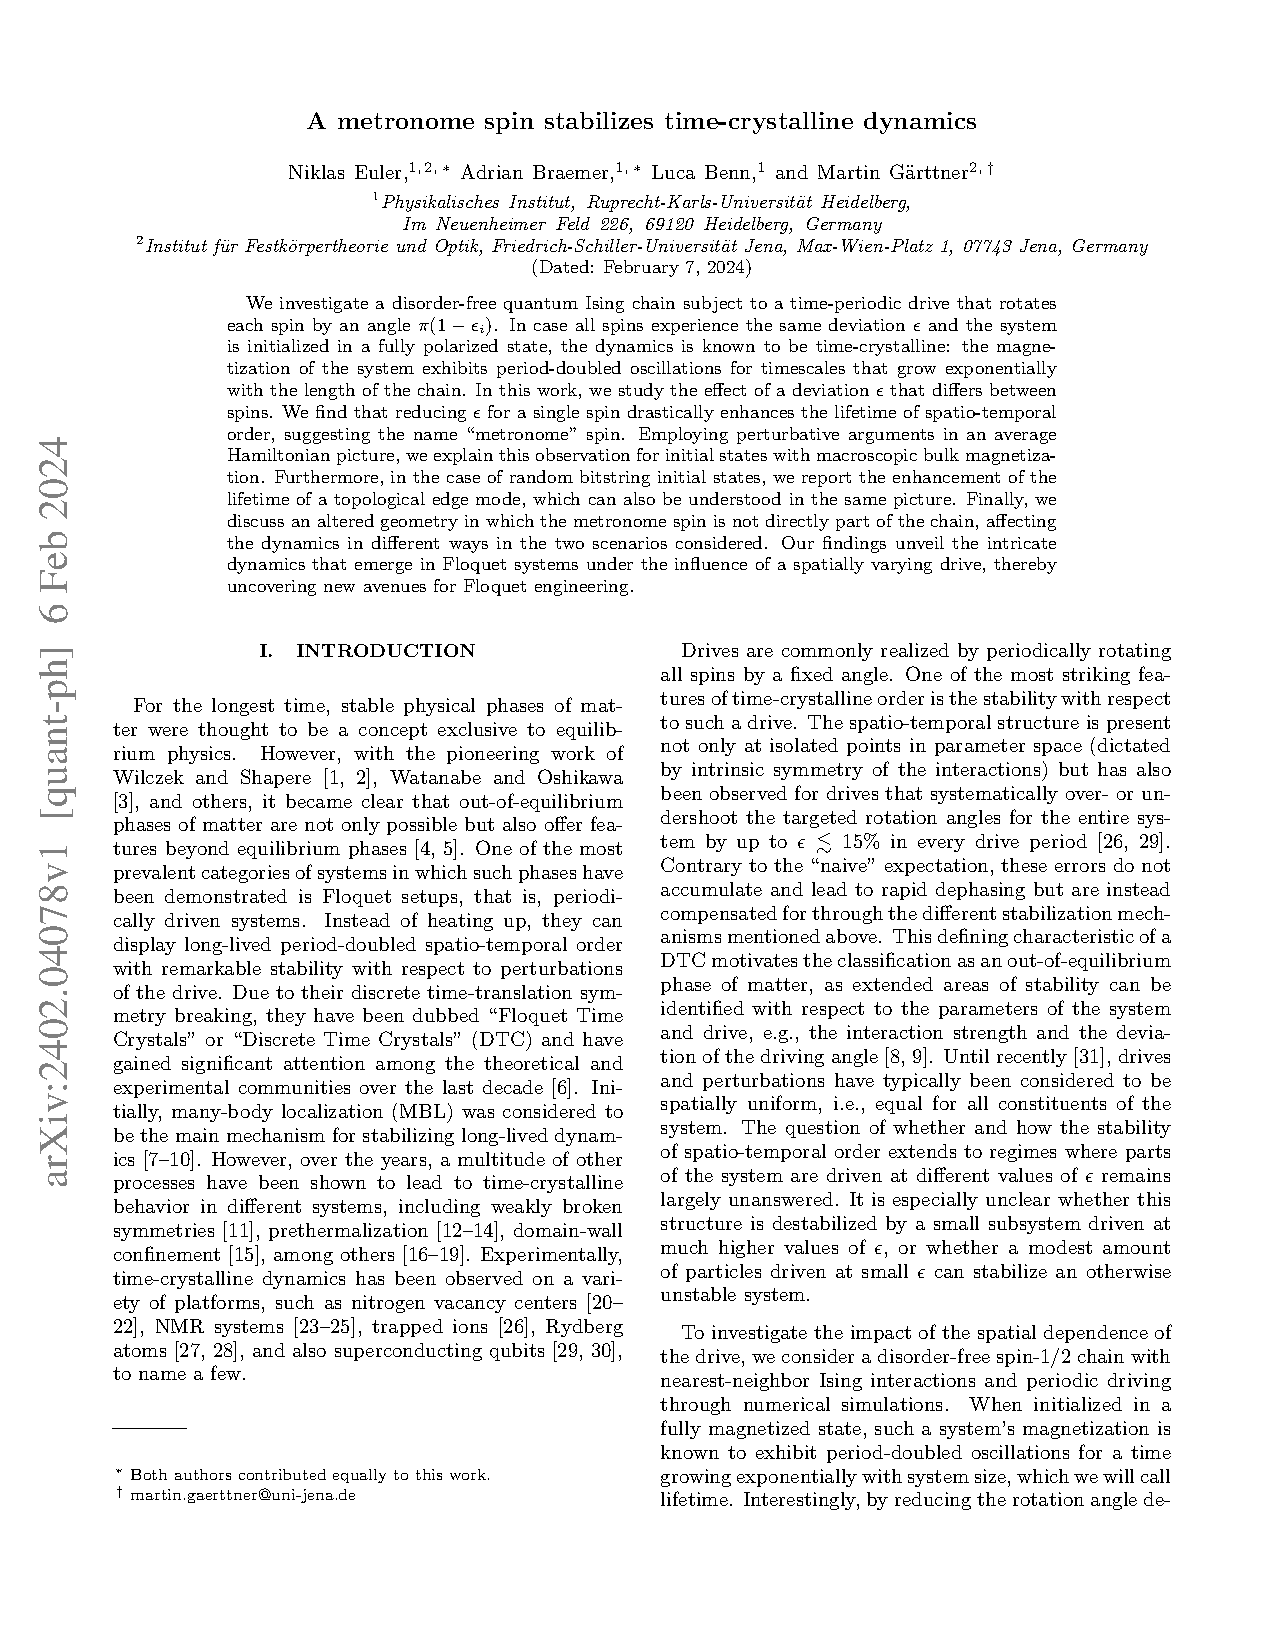
\includepdf[pages=-]{pub-Euler2024-MetronomeSpin}